\hypertarget{indicators}{\section{Indicators}}
\label{sec:indicators}
We define \numindicators indicators that comprehensively characterize transparency for foundation model developers.
To select these indicators, we compiled relevant concepts raised across past scientific literature as well as concerns animated by public discourse on foundation models and other digital technologies. In \refapp{indicators} we provide specific references for each indicator, and these references advocate for increased transparency and information sharing related to the indicator in question.
We derived a concrete set of indicators from this literature, engaging external researchers to converge on the final list of \numindicators (see \reffig{indicators}).
These indicators cover each dimension of the foundation model supply chain, from the data, compute, and labor required to build foundation models to model evaluations and developers' policies to restrict their use. 
We divide our indicators into three broad domains as described in \reffig{supply-chain}: indicators that are \textit{upstream} of the model, indicators that relate to the \textit{model} itself, and indicators that are \textit{downstream} of the model.

\hypertarget{upstream-indicators}{\subsection{Upstream indicators}}
\label{sec:upstream-indicators}
The upstream indicators identify the \emph{ingredients and processes} involved in building a foundation model. 
There are \numupstreamindicators upstream indicators, which we further taxonomize into the following \numupstreamsubdomains subdomains:

-  \textbf{\data (10 indicators).}
- Assesses transparency regarding the size and composition of the data used to build the model; the creators whose content is present in the data; and any steps to curate or augment the data.
- These indicators also address transparency regarding the inclusion of personal, copyrighted, or licensed data.
-  \textbf{\labor (7 indicators).}
- Assesses transparency regarding the use of human labor in producing the data used to build the model, including the wages, labor protections, employer, and geographic distribution of workers who contributed to data annotation and curation.
- These indicators also address transparency regarding the third parties that foundation model developers partnered with to construct their models.
-  \textbf{\dataaccess (2 indicators).}
- Assesses the scope of data access given to external parties.
-  \textbf{\compute (7 indicators).}
- Assesses transparency regarding the hardware and computation used to build the model, as well as the resulting energy use and environmental impacts.
-  \textbf{\methods (4 indicators).}
- Assesses basic technical specifications for the model's training stages and objectives, as well as the software frameworks and dependencies used.
-  \textbf{\datamitigations (2 indicators).}
- Assesses transparency regarding steps taken to mitigate data privacy and copyright concerns.

\begin{figure}
\centering
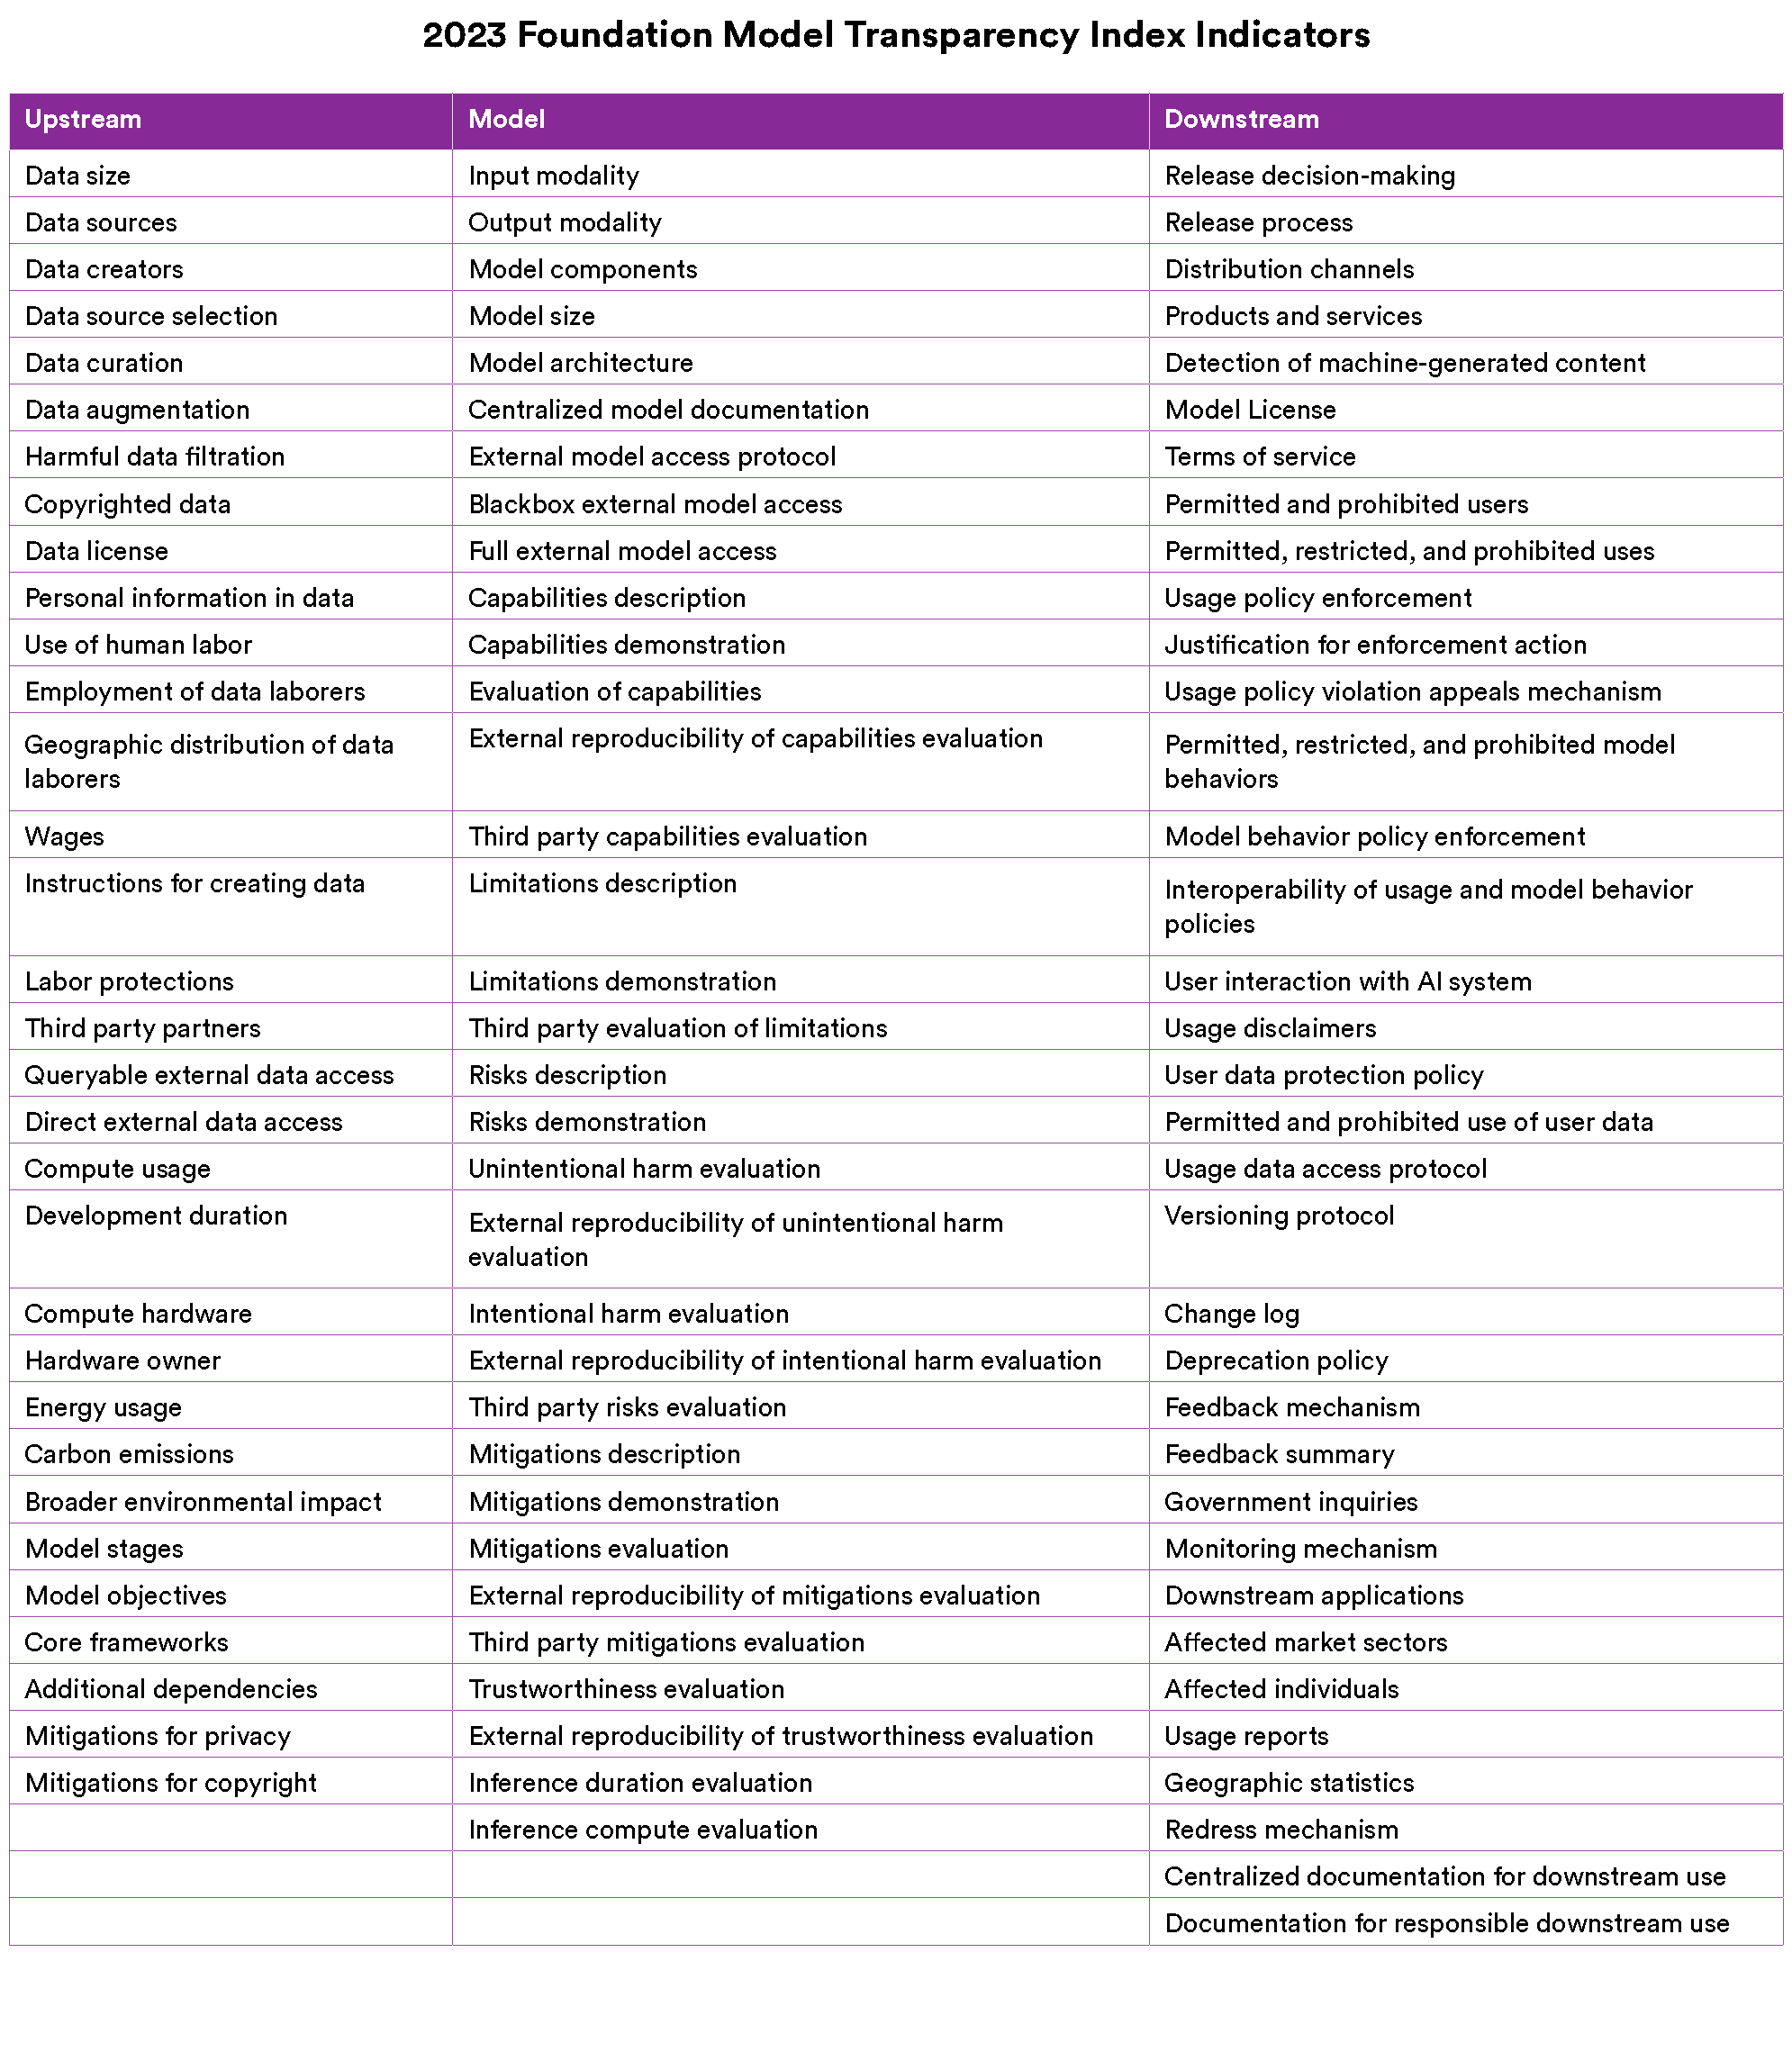
\includegraphics[keepaspectratio, height=\textheight, width=\textwidth]{figures/indicators_list.pdf}
\caption{\textbf{Indicators.} The \numindicators indicators of the \projectname spanning the \numdomains domains: upstream, model, and downstream.
% Would be good to remove horizontal lines
}.
\label{fig:indicators}
\end{figure}

\begin{figure}
\centering
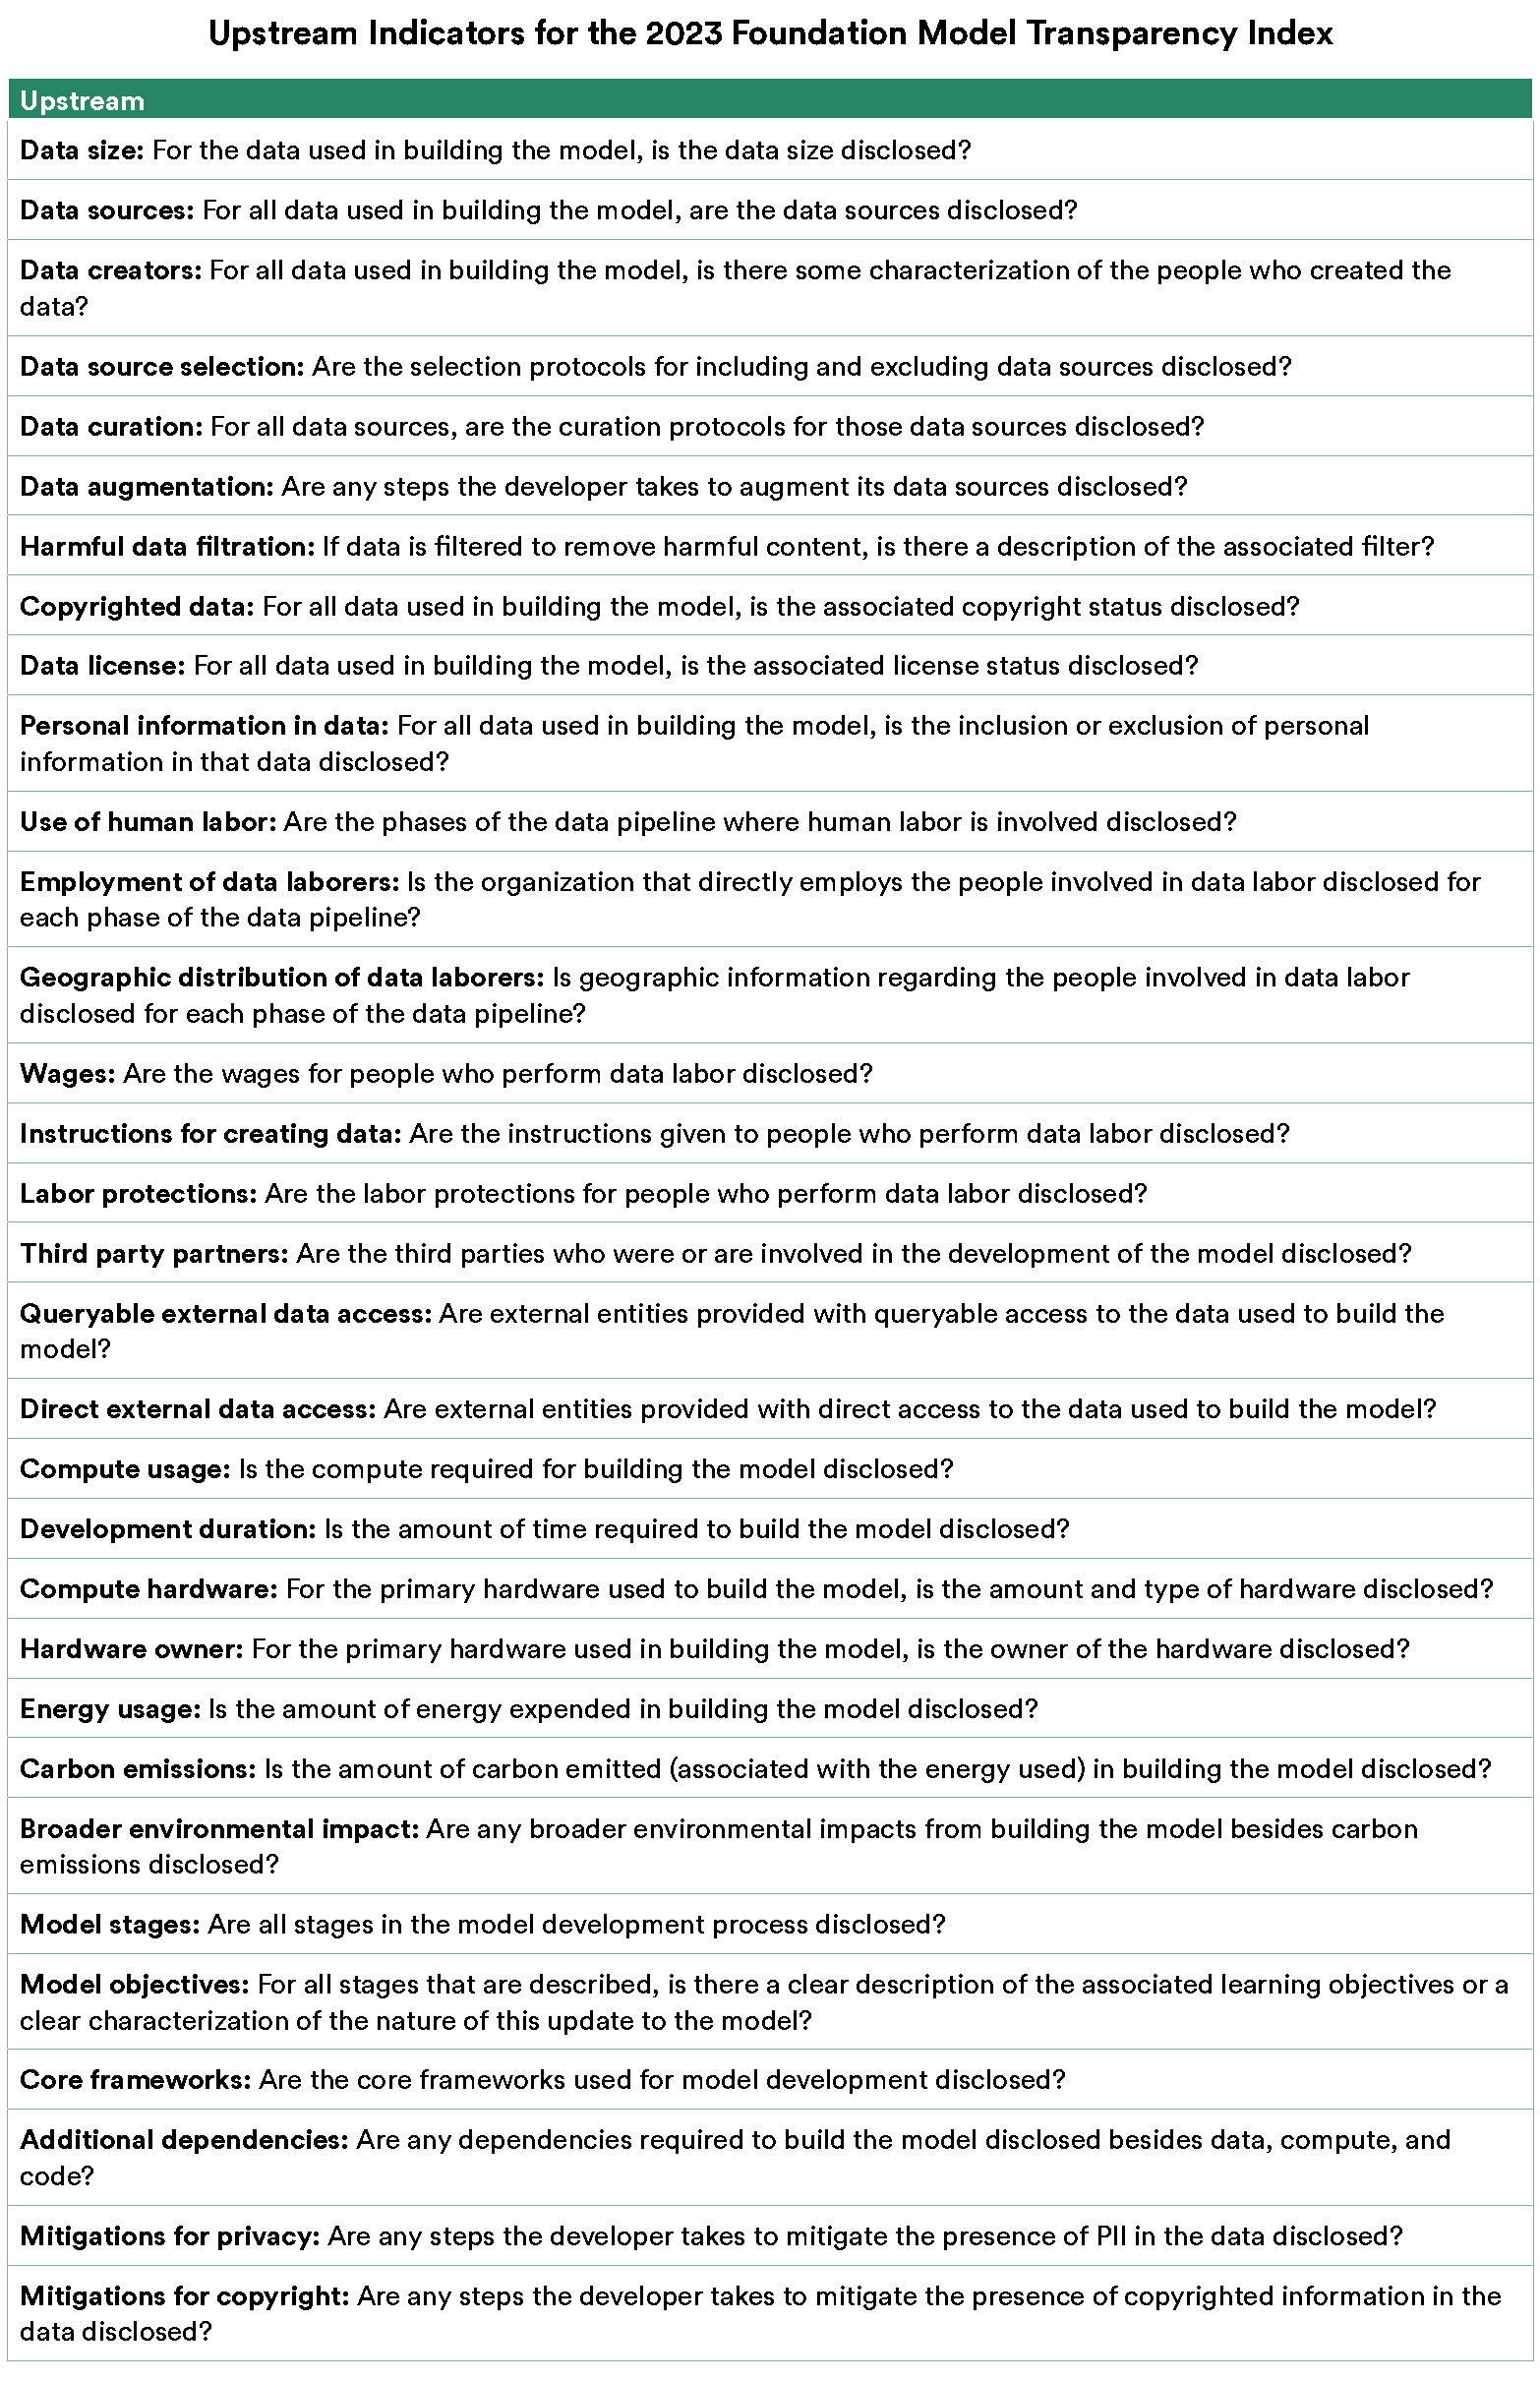
\includegraphics[keepaspectratio, height=\textheight, width=\textwidth]{figures/indicators_list_upstream.pdf}
\caption{\textbf{Upstream Indicators.} The \numupstreamindicators upstream indicators that span \data, \labor, \dataaccess, \compute, \methods, and \datamitigations.}
\label{fig:upstream-indicators}
\end{figure}

\noindent We depict the upstream indicators in \reffig{upstream-indicators}.
Researchers have widely advocated for greater transparency in relation to \data and \dataaccess \citep{bender-friedman-2018-data, gebru2018datasheets, hutchinson2021towards, dodge2021c4, bandy2021addressing} as a means for contextualizing model capabilities ~\citep{sambasivan2021everyone, longpre2023pretrainer} and risks related to privacy, bias, and copyright ~\citep{buolamwini2018gender,bender2021dangers, kandpal2022deduplicating,sobel2017artificial}.
\labor indicators uplift concerns related to labor practices, include irresponsible or exploitative use of human labor ~\citep{gray2019ghost, crawford2021atlas, hao2023cleaning, kittur2013future, dzieza2023ai, west2019data}.
\compute indicators relate to concerns around the high computational cost and energy expenditure associated with building foundation models, which can result in environmental harm \citep{lacoste2019quantifying,strubell2019energy,schwartz2020green,patterson2021carbon,bender2021dangers,henderson2020towards,luccioni2023counting,vipra2023comments}.
\datamitigations indicators also relate to the growing legal and sociotechnical concerns over data privacy, copyright, and licensing \citep{henderson2023foundation, brown2022does, lee2023talkin,genlaw2023,tremblay2023openai}.

\hypertarget{model-indicators}{\subsection{Model indicators}}
\label{sec:model-indicators}
The model indicators identify the \emph{properties and function} of the foundation model. 
There are \nummodelindicators model indicators, which we further taxonomize into the following \nummodelsubdomains subdomains:
-  \textbf{\modelbasics (6 indicators).}
- Assesses transparency regarding fundamental information about the model such as modalities, size, and architecture as well as the presence of centralized model documentation.
-  \textbf{\modelaccess (3 indicators).}
- Assesses the scope of model access given to external entities.
-  \textbf{\capabilities (5 indicators).}
- Assesses transparency regarding the capabilities of the model, including evaluations.
-  \textbf{\limitations (3 indicators).}
- Assesses transparency regarding the limitations of the model, including evaluations.
-  \textbf{\risks (7 indicators).}
- Assesses transparency regarding the risks of the model, including evaluations, with specific focus on both unintentional harm (\eg bias) and intentional harm (\eg fraud).
-  \textbf{\modelmitigations (5 indicators).}
- Assesses transparency regarding model-level mitigations, including evaluations of their efficacy.
-  \textbf{\trustworthiness (2 indicators).}
- Assesses transparency regarding the trustworthiness of the model, including evaluations.
-  \textbf{\inference (2 indicators).}
- Assesses transparency regarding standardized inference with the model.

\begin{figure}
\centering
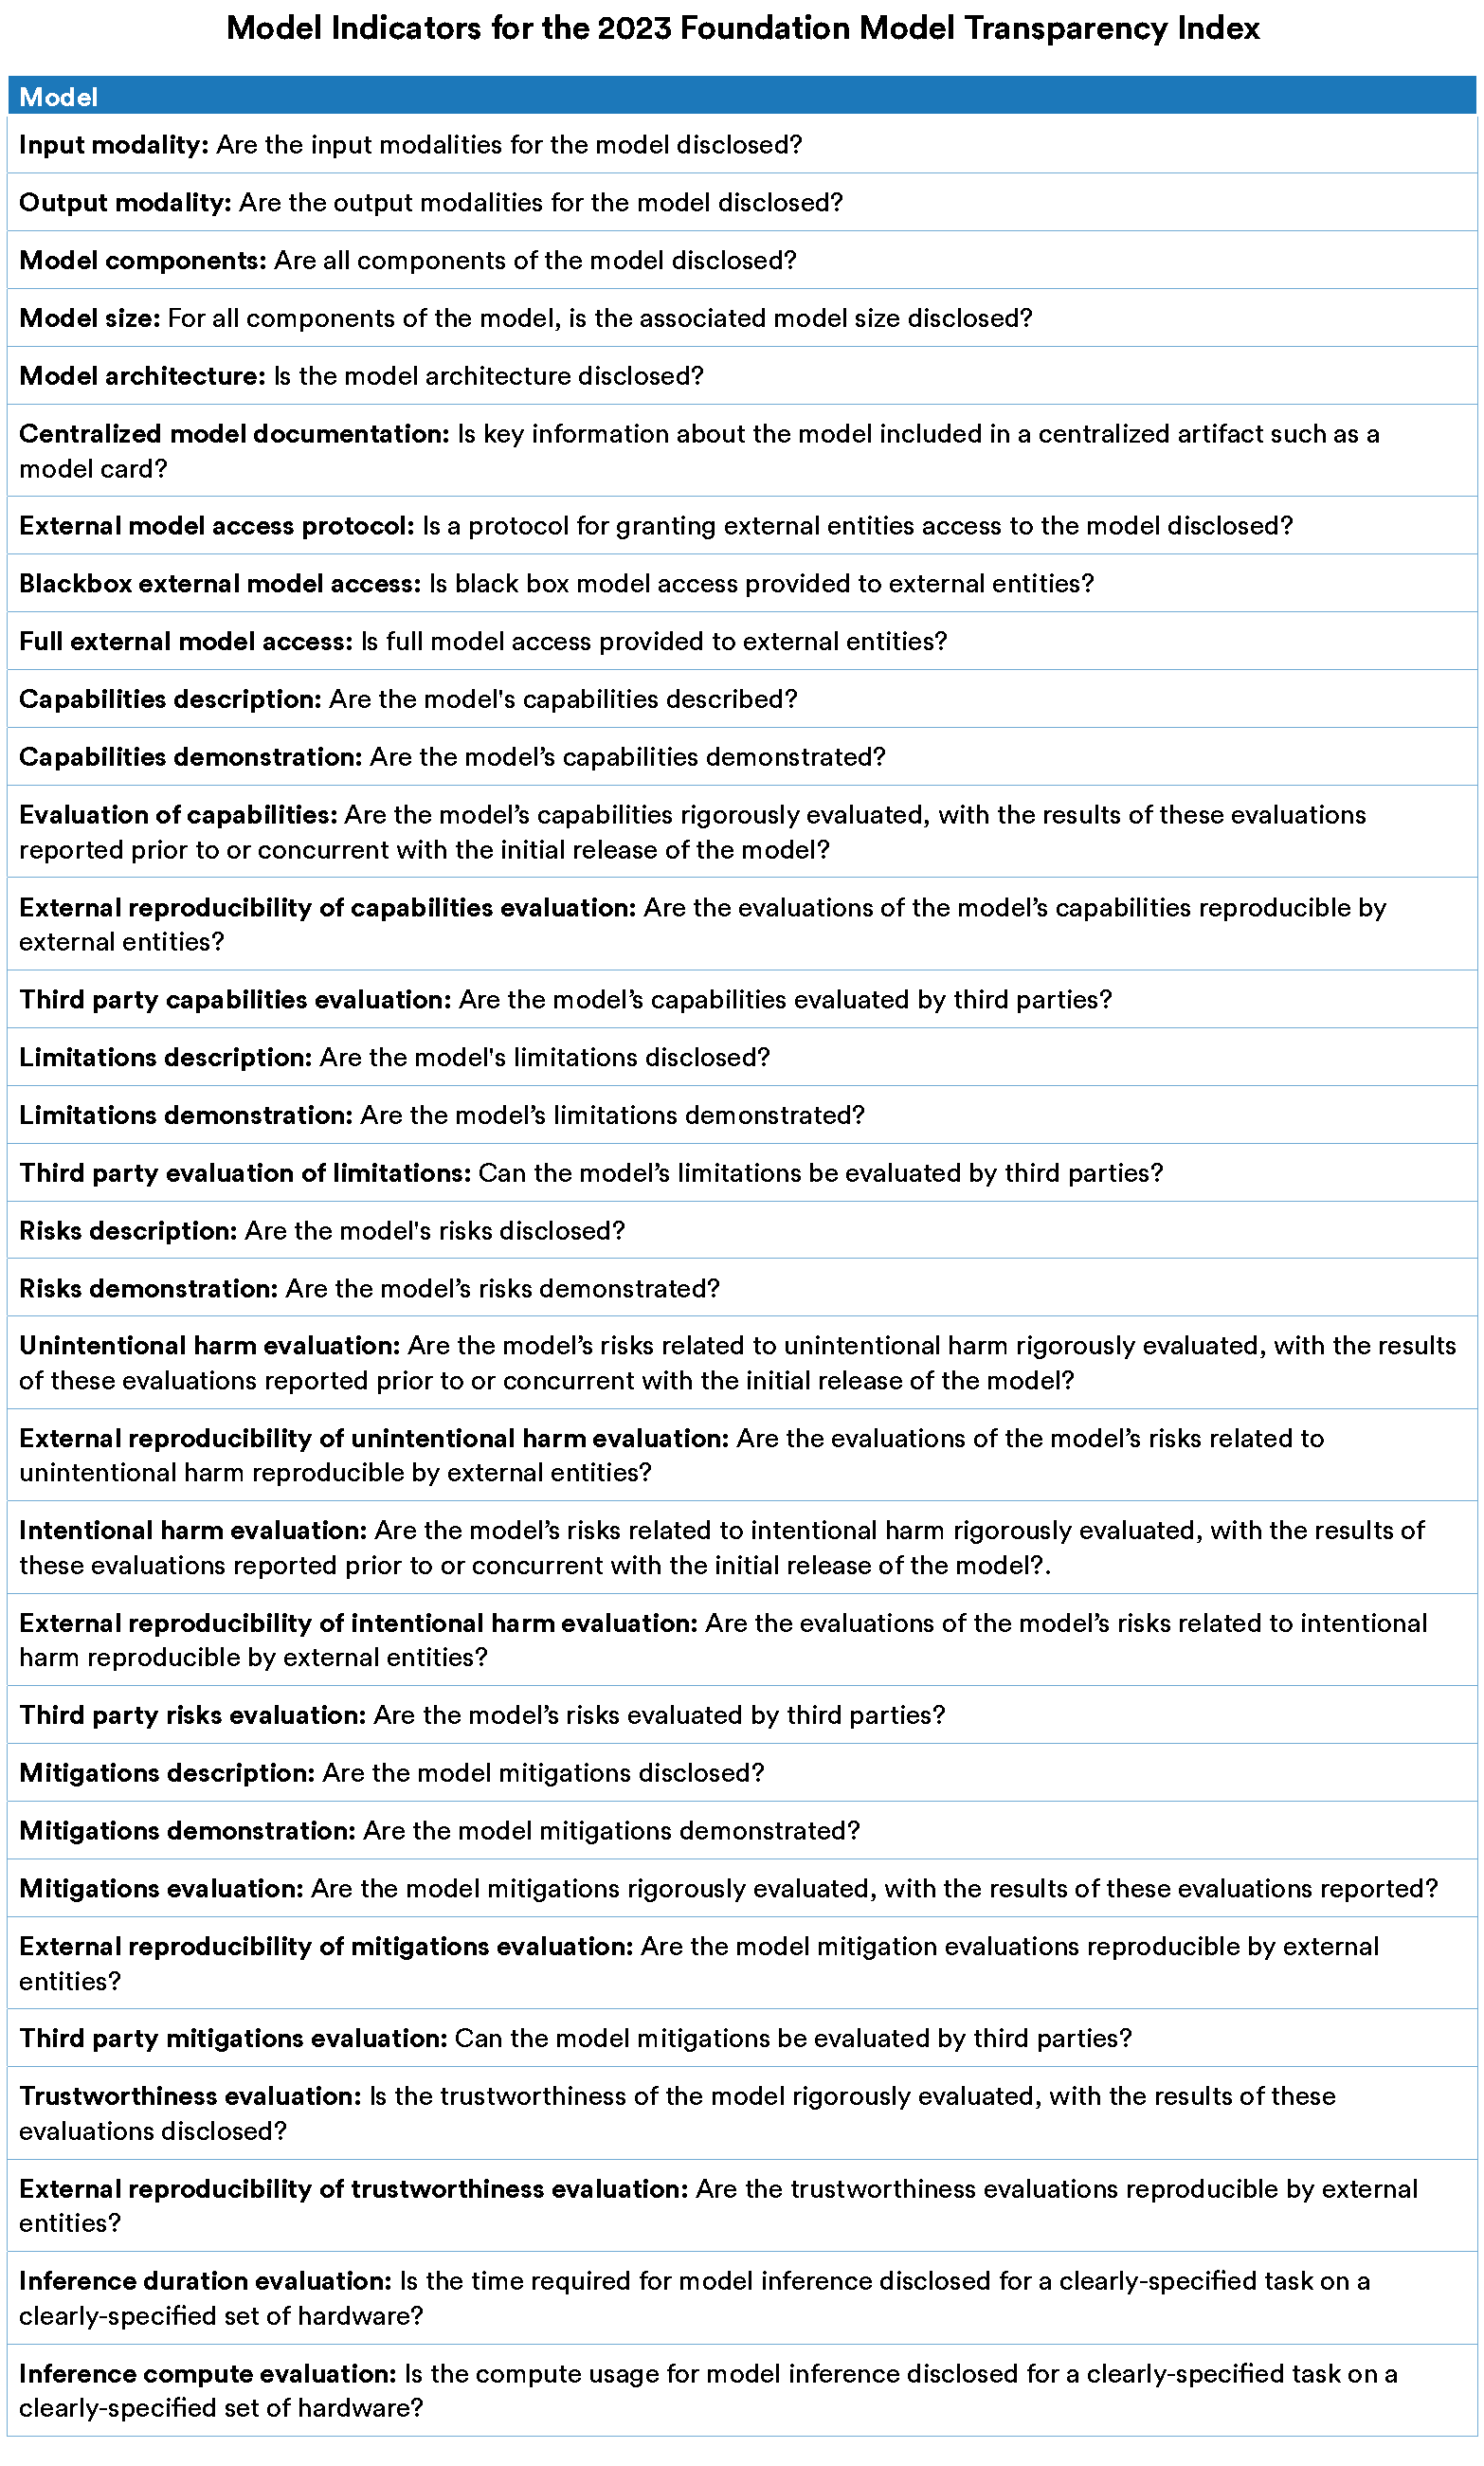
\includegraphics[keepaspectratio, height=\textheight, width=\textwidth]{figures/indicators_list_model-1.pdf}
\caption{\textbf{Model Indicators.} 
The \nummodelindicators model indicators that span \modelbasics, \modelaccess, \capabilities, \limitations, \risks, \modelmitigations, \trustworthiness, and \inference.}
\label{fig:model-indicators}
\end{figure}

\noindent 
We depict the model indicators in \reffig{model-indicators}.
\modelbasics indicators refer to fundamental information that is expected by model documentation standards \citep{mitchell2019model, crisan2022interactive, bommasani2023ecosystem} and, historically, have been reliably reported in the release of machine learning models. 
\modelaccess indicators reflect literature tied to the spectrum of model release and the associated differences in external access \citep{solaiman2019release, sastry2021release, shevlane2022structured, liang2022norms, solaiman2023gradient}. 
The indicators on \capabilities, \limitations, \risks and \modelmitigations are motivated by a common understanding that these factors jointly influence the societal impact of machine learning models and AI systems \citep{tabassi2023airmf, weidinger2023sociotechnical}. 
For these subdomains, the description and demonstration indicators gauge whether there is some non-technical articulation and legibility of these concepts, primed by concerns surrounding public understanding of foundation models.\footnote{See \url{https://www.gov.uk/government/publications/public-perceptions-towards-the-use-of-foundation-models-in-the-public-sector}.} 
To make these assessments more rigorous, the evaluation indicators build on the extensive tradition of evaluation in AI spanning iconic benchmarks like ImageNet \citep{deng2009imagenet}, broader benchmarks like SuperGLUE \cite{wang2019superglue}, and extensive meta-benchmarks like LM-Harness, BIG-bench, HELM and BEHAVIOR \citep{gao2021harness, srivastava2022bigbench, liang2023holistic, srivastava2021behavior}. 
Indicators assessing evaluations also highlight the importance of reproducibility \citep{lipton2019troubling, kapoor2023reforms, kapoor2023leakage}\footnote{See the ML Reproducibility challenge: \url{https://paperswithcode.com/rc2022}, CodaLab worksheets for reproducible ML: \url{https://worksheets.codalab.org/}, and Joelle Pineau's reproducibility checklist: \url{https://www.cs.mcgill.ca/~jpineau/ReproducibilityChecklist.pdf}.} and independent assessment \citep{sandvig2014auditing, raji2019actionable, metaxa2021audit, costanzachock2022audit, raji2022audit, raji2022mozilla, lam2022user, weidinger2023sociotechnical}, which enable open science and external verification of developers' claims about their models.
In the case of risks, finer distinctions between unintentional harms (\eg biases, toxicity) and intentional harms (\eg disinformation, fraud) build on harm taxonomies \citep{bender2021dangers, bommasani2021opportunities, weidinger2021ethical, nist2023airmf, weidinger2023sociotechnical}.
Indicators on trustworthiness and inference are especially motivated by the Trustworthy ML Initiative\footnote{\url{https://www.trustworthyml.org/}} and MLPerf \citep{reddi2020mlperf} respectively, among other works \citep{brundage2020toward, cammarota2020trustworthy, kumar2020trustworthy, liu2022trustworthy, shneiderman2020bridging, patterson2021carbon, narayanan2023cheaply}.

\hypertarget{downstream-indicators}{\subsection{Downstream indicators}}
\label{sec:downstream-indicators}
The downstream indicators identify the \emph{use} of the foundation model, including details about its \textit{release}.
There are \numdownstreamindicators downstream indicators, which we further taxonomize into the following \numdownstreamsubdomains subdomains:

-  \textbf{\distribution (7 indicators).}
- Assesses transparency regarding the release process, the distribution channels for the model, and the products and services that arise through internal use.
- Additionally, this subdomain assesses the presence of model licenses, terms of service, and mechanisms for detecting model-generated content.
-  \textbf{\usagepolicy (5 indicators).}
- Assesses transparency regarding the developer's acceptable use policy such as restrictions on specific uses or users, as well as transparency regarding how it enforces such policies.
-  \textbf{\modelbehaviorpolicy (3 indicators).}
- Assesses transparency regarding the developer's policy on acceptable and unacceptable model behavior as well as transparency regarding enforcement of this policy and expectations in the event of usage policy violations.
-  \textbf{\interface (2 indicators).}
- Assesses transparency in the user interface for the developer's flagship distribution channel, if the channel includes a user interface.
-  \textbf{\dataprotection (3 indicators).}
- Assesses transparency regarding the developer's policies with respect to user data protection, such as how data is stored, shared, and accessed.
-  \textbf{\updates(3 indicators).}
- Assesses transparency regarding the developer's versioning protocol, change log, and deprecation policy.
-  \textbf{\feedback (3 indicators).}
- Assesses transparency regarding mechanisms for reporting feedback on the model, summaries of feedback received, and related government inquiries.
-  \textbf{\impact (7 indicators).}
- Assesses transparency regarding the downstream impact of the model on society, such as affected market sectors, individuals, and geographies.
- Additionally, this subdomain assesses transparency regarding downstream applications, usage statistics, and mechanisms for monitoring usage as well as providing redress in the event of harm to users.
-  \textbf{\documentation (2 indicators).}
- Assesses the presence of centralized documentation for downstream use and documentation for responsible downstream use.

\begin{figure}
\centering
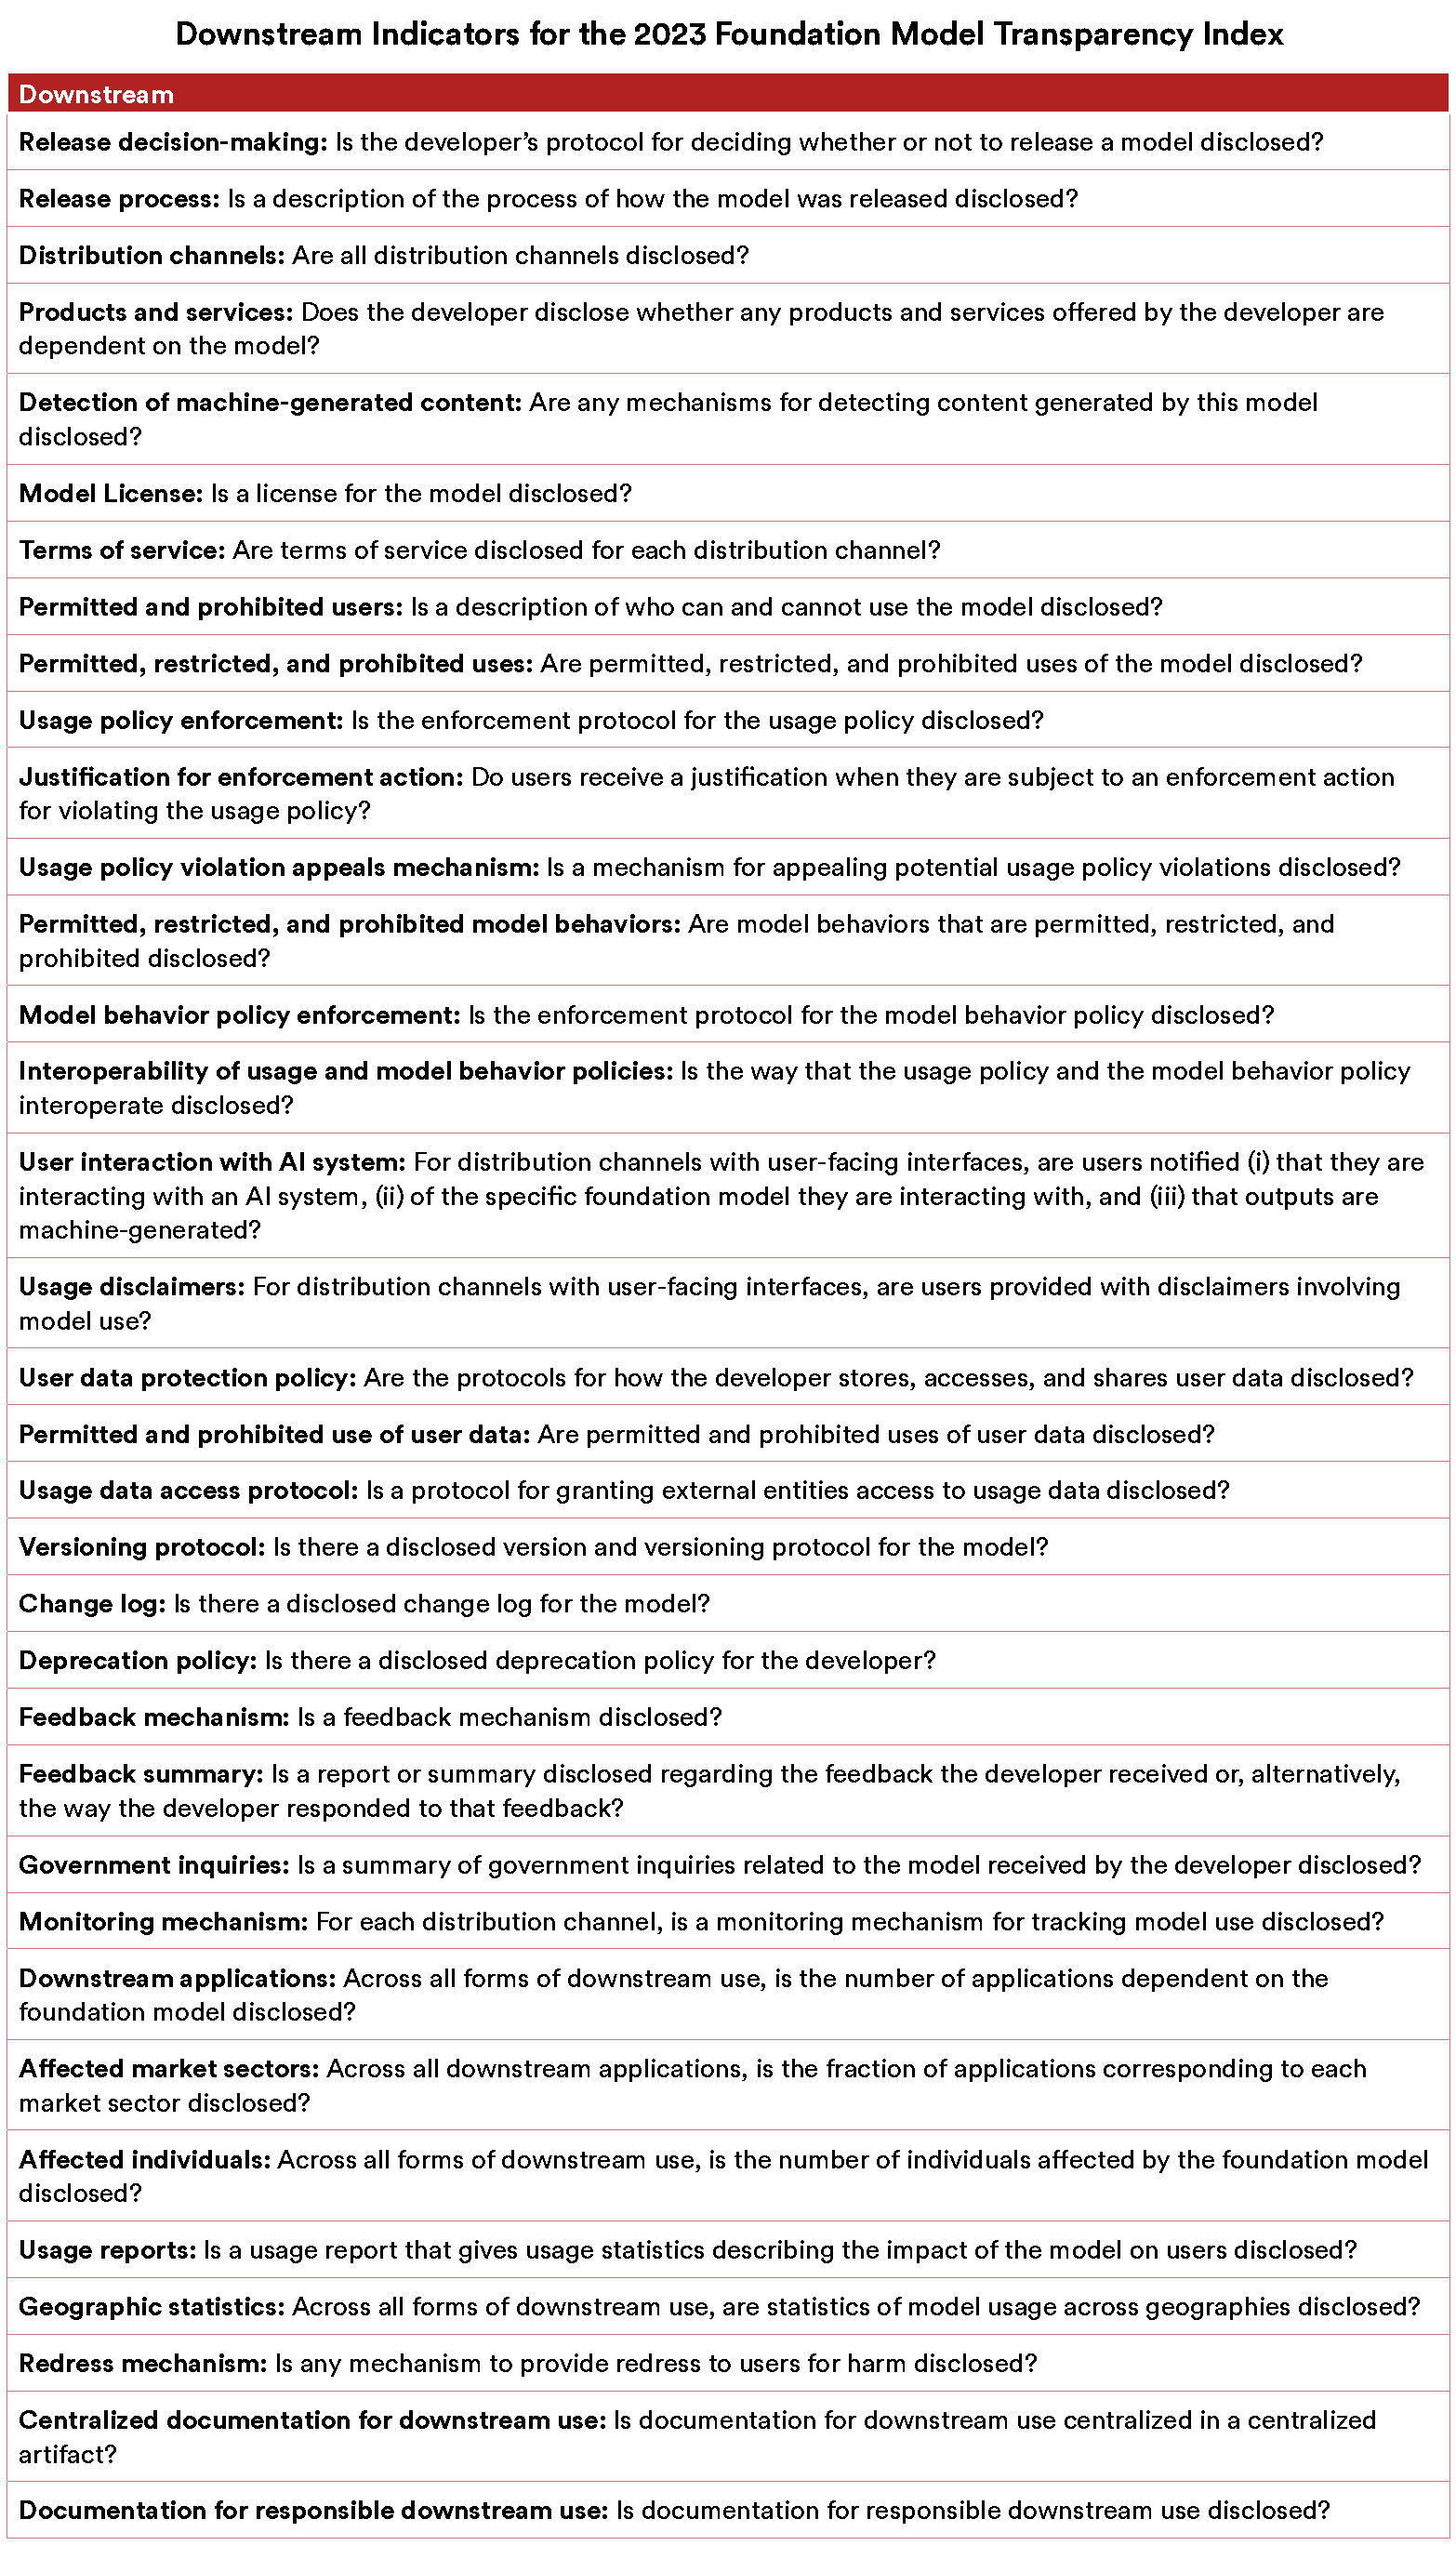
\includegraphics[keepaspectratio, height=\textheight, width=\textwidth]{figures/indicators_list_downstream.pdf}
\caption{\textbf{Downstream Indicators.} 
The \numdownstreamindicators downstream indicators that span \distribution, \usagepolicy, \modelbehaviorpolicy, \interface, \dataprotection, \updates, \feedback, \impact, and \documentation.}
\label{fig:downstream-indicators}
\end{figure}

\noindent We depict the downstream indicators in \reffig{downstream-indicators}.
Given that foundation models are the basis for a downstream supply chain \citep{bommasani2021opportunities}, the distribution indicators are informed by the literature on AI supply chains \citep{bommasani2023ecosystem, vipra2023concentration, cen2023supplychain, cobbe2023supply, widder2023thinking, brown2023allocating} and release practices \citep{liang2022thetime, solaiman2023gradient, henderson2023foundation, pmlr-v202-kirchenbauer23a, Kuditipudi2023RobustDW, liesenfeld2023opening}. 
Usage policy indicators draw from company publications on responsible model deployment \cite{cohere2022} as well precedents from social media. 
Model behavior policy indicators are rooted in literature that discusses AI behavior and trustworthiness, risks, mitigation and refusal \cite{kumar2022language, weidinger2021ethical, brundage2020toward, cammarota2020trustworthy, kumar2020trustworthy, liu2022trustworthy, reuter2023im}. 
User interface indicators are derived from research on safety by design and human-centered user interfaces \cite{qiaosi2023ux, nakao2022responsible}. 
User data protection indicators are inspired by policy recommendations on user data minimization, privacy, preservation, protection and contextual integrity \cite{eu2016, brown2022does,vipra2023, winograd2023privacy, nissenbaum2004contextual, king2020privacy, mulligan2017privacy}.
Model updates indicators stem from work focused on adequately updating systems and version control of AI systems \citep{sathyavageesran2022privacy, hashesh2023version, chen2023chatgpts}. 
For feedback, impact and downstream documentation, the indicators were motivated by the literature on algorithmic auditing \cite{liang2022thetime, solaiman2023gradient, raji2022audit} as well as transparency reporting practices for social media.\footnote{See \url{https://www.tspa.org/curriculum/ts-fundamentals/transparency-report/}, \url{https://transparencyreport.google.com/} and \url{https://transparency.fb.com/reports/}.}

\paragraph{Note on assessment of indicators.}
We assess each indicator based on the information that developers share publicly about their flagship foundation models and their practices that apply to these models. 
Our standard for awarding points on an indicator is that the developer must explicitly state the information related to the indicator in its documentation, or it must explicitly point to the information in its documentation.
This implies that if developers are overly vague or do not link to a key external document for a particular indicator then they do not receive a point.
In addition, if developers explicitly state in their documentation that they \emph{do not} carry out a specific action related to an indicator (\eg they do not have a mechanism for users to provide feedback) then we generally award a point for that indicator.
We note that this is exceedingly rare and that, in general, developers share little information about the actions they do or do not take in the process of developing and deploying foundation models.

\paragraph{Note on inclusion of deployment.}
Our view of transparency is expansive, considering the broader supply chain beyond just foundation models.
As we discuss in \refsec{background-transparency}, existing conceptualizations of transparency in AI often consider upstream resources (especially data) in addition to machine learning models.
But these works and broader public discourse usually do not foreground the downstream use and impact of AI, even though this is the most direct way in which AI affects society.
To this end, we include the entire downstream domain to bring greater attention to this vital topic.

In particular, while we are assessing foundation model developers, we assess them in relation to distribution channels and other factors that determine their downstream impact.
At present, we recognize that characterizing the downstream impact of foundation models may be challenging, especially for open model developers.
By releasing a model openly, developers may cede the ability to easily monitor the model's downstream use and impact.
Open model developers can be fully transparent by being clear about the ways in which they do or do not monitor downstream use and impact.
In addition, we believe in the potential for greater coordination between foundation model developers and distribution channels to increase transparency; for example, distribution channels could supply information about how the model is used to the foundation model developer.
Partnerships with distribution channels that promote transparency provide a promising means for all foundation model developers to share more information about the impact their models have on society.